\documentclass[11pt]{article}

\usepackage[margin=2.5cm]{geometry}
\usepackage{amsmath}
\usepackage{amssymb}
\usepackage{graphicx}
\usepackage{booktabs}
\usepackage{hyperref}

\graphicspath{{../../plots/c000_hod484/}}

\newcommand{\Mpch}{\,h^{-1}\,\mathrm{Mpc}}

\title{Technical note: the zero crossing of the two-point correlation
function in environment-split clustering}
\author{ASTRA clustering project}
\date{June 2026}

\begin{document}
\maketitle

\begin{abstract}
We measure the two-point correlation function (2PCF) of an AbacusSummit
HOD galaxy catalog, split by cosmic-web environment with the ASTRA
classification.  All our statistics --- the full-sample auto-correlation,
the environment-quantile auto-correlations, and the cross-correlations with
the full sample --- change sign at the same scale, $s \simeq 120\Mpch$.
This note explains why this zero crossing exists, why its location is
shared by all linearly biased tracers, and how our finite subbox volume
shifts it.  The crossing scale is a known cosmological standard ruler
related to the horizon size at matter--radiation equality
\cite{prada2011}.
\end{abstract}

\section{Why the correlation function must cross zero}

The correlation function is the Fourier transform of the power spectrum,
\begin{equation}
\xi(r) \;=\; \frac{1}{2\pi^{2}} \int_{0}^{\infty} dk\, k^{2} P(k)\,
j_{0}(kr),
\label{eq:xi_from_pk}
\end{equation}
where $j_{0}(x) = \sin x / x$ is the spherical Bessel function.  The
inverse relation at $k=0$ gives a sum rule,
\begin{equation}
P(k\!=\!0) \;=\; \int \xi(r)\, d^{3}r .
\label{eq:sumrule}
\end{equation}
For a primordial spectrum $P(k) \propto k^{n_s}$ with $n_s > 0$, the
left-hand side of Eq.~(\ref{eq:sumrule}) vanishes.  The strong positive
correlations at small $r$ must therefore be compensated by a shallow
negative tail at large $r$.  In other words, every overdense region sits
inside a slightly underdense larger environment.  The scale where
$\xi(r)$ changes sign is set by the turnover of $P(k)$, which reflects
the size of the horizon at matter--radiation equality.  For Planck-like
parameters the linear-theory crossing lies at $r_{0} \approx
125$--$130\Mpch$, just outside the BAO peak.  Reference \cite{prada2011}
showed with $N$-body simulations that this crossing is stable against
nonlinear evolution, redshift-space distortions, and galaxy bias, and
proposed it as a standard ruler for the equality horizon.  A related,
template-free ruler built from features of $\xi(r)$ near the BAO range is
the ``linear point'' \cite{anselmi2016,anselmi2018}.

\section{Why all biased tracers cross at the same scale}

At leading order, a galaxy sample $g$ with linear bias $b$ follows the
matter field,
\begin{equation}
\xi_{g}(r) \;=\; b^{2}\, \xi_{m}(r),
\qquad
\xi_{g_1 g_2}(r) \;=\; b_{1} b_{2}\, \xi_{m}(r).
\label{eq:bias}
\end{equation}
In redshift space, linear theory (Kaiser) modifies only the amplitude of
the monopole,
\begin{equation}
\xi_{0}(s) \;=\;
\left( b^{2} + \tfrac{2}{3} b f + \tfrac{1}{5} f^{2} \right)
\xi_{m}(s),
\label{eq:kaiser}
\end{equation}
with $f$ the linear growth rate.  Equations~(\ref{eq:bias}) and
(\ref{eq:kaiser}) rescale $\xi$ but cannot move its zero.  As a
consequence, all tracers with scale-independent bias must cross zero at
the same comoving scale, at any redshift.  This makes the common crossing
a simple consistency test: if an environment-selected sample crossed at a
clearly different scale, this would signal scale-dependent bias.

\section{Our setup}

We use one AbacusSummit base box (cosmology \texttt{c000}, phase
\texttt{ph000}, side $2000\Mpch$) \cite{maksimova2021}, populated with an
LRG-like HOD at $z=0.5$ (catalog \texttt{hod484} from the EMC emulator
set, $4\times10^{6}$ galaxies).  Positions include redshift-space
distortions along the $z$ axis.  We divide the box into a $4\times4\times4$
grid of 64 subboxes of $500\Mpch$ and treat each subbox as an independent
volume with open boundaries.

In each subbox, the ASTRA method classifies the local environment.  We
build a Delaunay triangulation over the union of the galaxies and an equal
number of uniform random points.  For every galaxy we count data
neighbours $n_{d}$ and random neighbours $n_{r}$ in the triangulation and
define the local density indicator
\begin{equation}
r_{\rm ASTRA} \;=\; \frac{n_{d} - n_{r}}{n_{d} + n_{r}} .
\label{eq:astra}
\end{equation}
Galaxies and randoms are then split independently into four quantiles of
$r_{\rm ASTRA}$ (Q1 = most underdense, Q4 = most overdense).  We measure
the 2PCF multipoles ($\ell = 0, 2$) with \texttt{pycorr}/\texttt{Corrfunc}
\cite{sinha2020} in 15 separation bins over $0 < s < 150\Mpch$, using the
Landy--Szalay estimator \cite{landy1993}
\begin{equation}
\hat{\xi} \;=\; \frac{DD - 2\,DR + RR}{RR},
\label{eq:ls}
\end{equation}
with a fixed catalog of uniform geometry randoms ($5\times$ the data).
The mean over the 64 subboxes gives the signal; the scatter gives the
cosmic variance.

\section{Results}

Figure~\ref{fig:full} shows the full-sample auto-correlation.
Figure~\ref{fig:auto} shows the auto-correlations of the four data and
random quantiles, and Figure~\ref{fig:cross} the cross-correlations of
each quantile with the full sample.  Table~\ref{tab:crossings} lists the
measured zero crossings of the monopole.  All statistics with a
positive-to-negative crossing agree on $s_{0} \simeq 117$--$123\Mpch$.
The Q1 cross-correlation is negative at small $s$ (underdense regions are
anti-biased) and approaches zero from below, so it has no such crossing.

\begin{table}[ht]
\centering
\begin{tabular}{lcc}
\toprule
Statistic & auto $s_{0}$ [$h^{-1}$Mpc] & cross with full $s_{0}$ [$h^{-1}$Mpc] \\
\midrule
Full sample & 123 & --- \\
Q1 (most underdense) & 135 & no $+\!\to\!-$ crossing \\
Q2 & 112 & 117 \\
Q3 & 123 & 123 \\
Q4 (most overdense) & 123 & 123 \\
\bottomrule
\end{tabular}
\caption{Zero crossings of the monopole, from the mean over 64 subboxes
of the \texttt{c000} (fiducial) run.  The statistical precision per bin
near the crossing is a few $h^{-1}$Mpc.}
\label{tab:crossings}
\end{table}

The common crossing is consistent with the linear-bias expectation of
Section~2.  Its location is a few $\Mpch$ \emph{inside} the linear-theory
value.  We attribute this to the integral constraint of the finite subbox:
the estimator of Eq.~(\ref{eq:ls}) measures clustering with respect to the
mean density of each $500\Mpch$ subbox, which biases the estimate low by
roughly the volume average
\begin{equation}
\hat{\xi}(s) \;\approx\; \xi(s) - \bar{\xi}_{V},
\qquad
\bar{\xi}_{V} = \frac{1}{V^{2}} \int_{V}\!\!\int_{V}
\xi(|\mathbf{x}-\mathbf{y}|)\, d^{3}x\, d^{3}y
\;\sim\; 10^{-3}.
\label{eq:ic}
\end{equation}
At $s \gtrsim 100\Mpch$ the true $|\xi|$ is of the same order as
$\bar{\xi}_{V}$, so the constraint pulls the apparent crossing inward and
deepens the negative tail.  Averaging over subboxes does not remove this
effect because it acts inside each subbox.  A measurement in the full
$2000\Mpch$ box would move the crossing back toward the linear-theory
value.

\begin{figure}[ht]
\centering
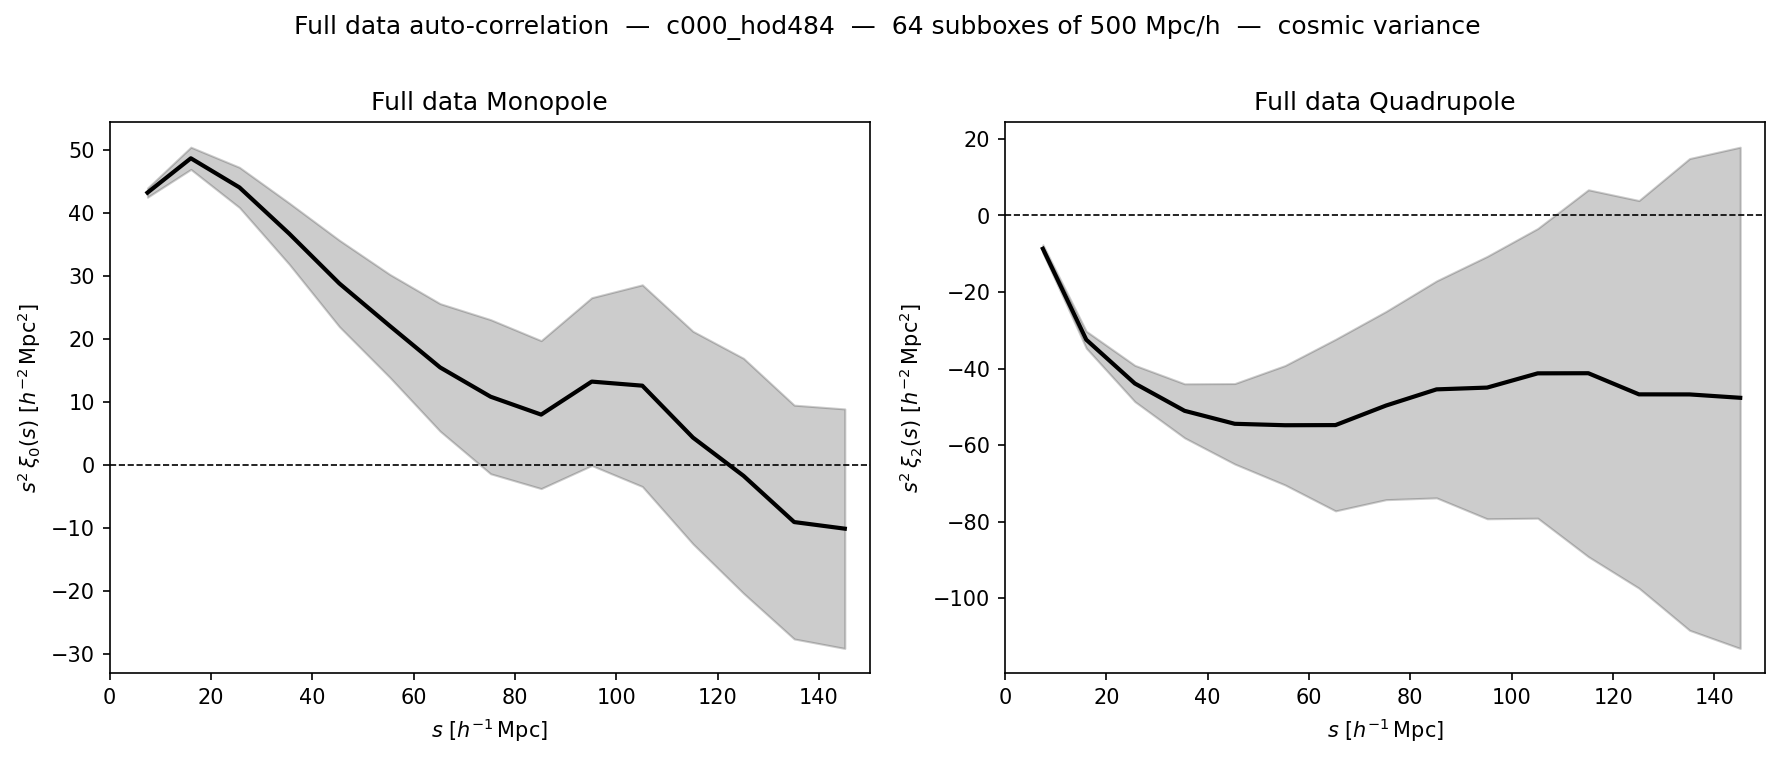
\includegraphics[width=0.95\textwidth]{subbox_full_data_autocorr.png}
\caption{Full-sample auto-correlation (monopole and quadrupole), mean
and $\pm1\sigma$ over 64 subboxes.  The monopole crosses zero at
$s \simeq 123\Mpch$.}
\label{fig:full}
\end{figure}

\begin{figure}[ht]
\centering
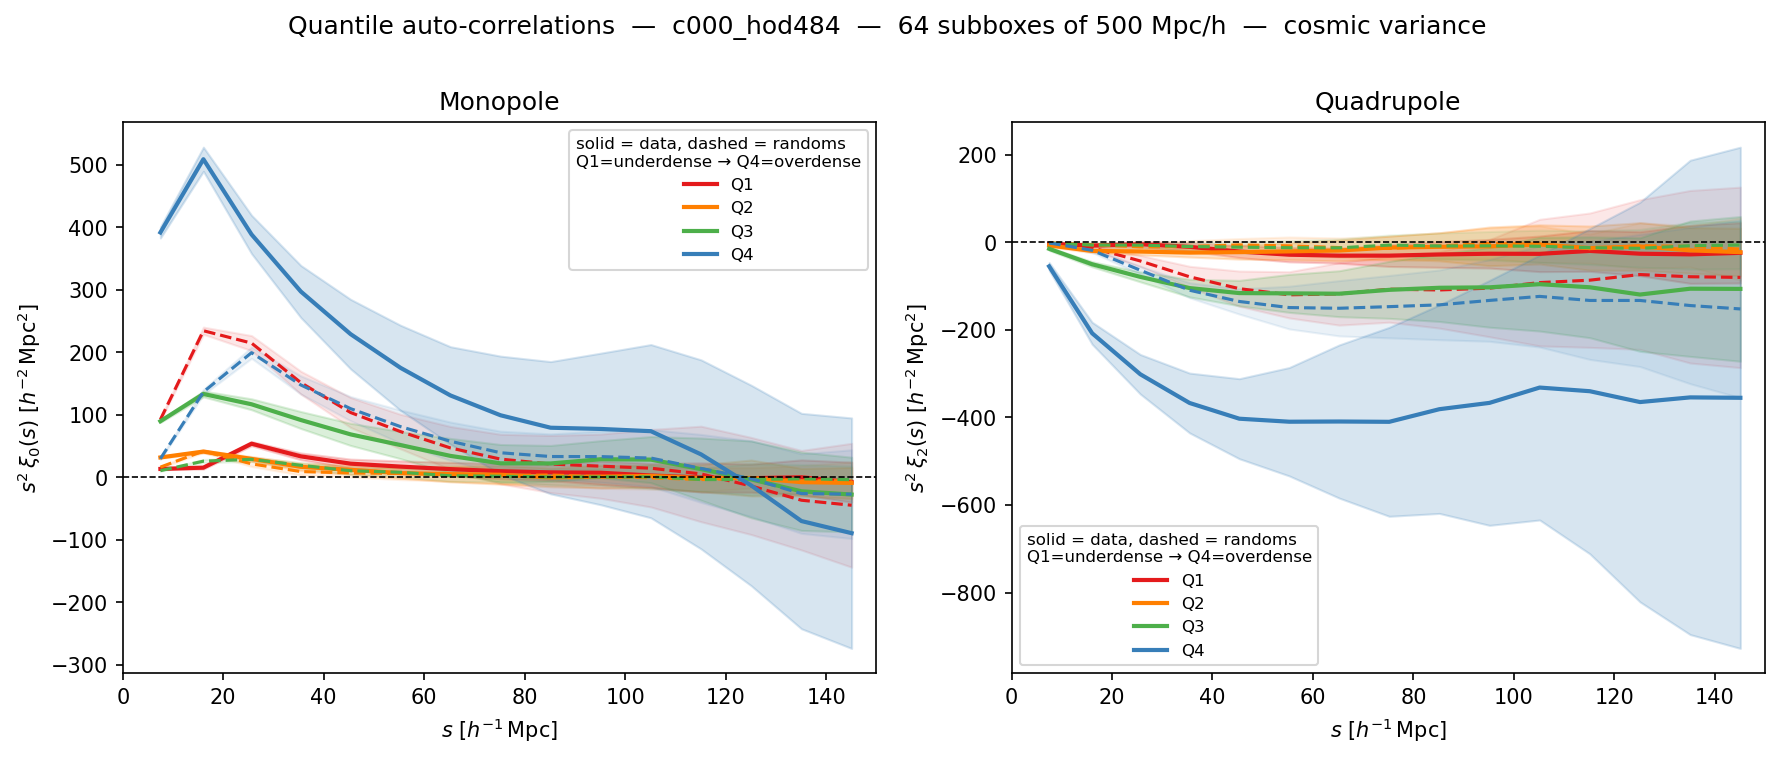
\includegraphics[width=0.95\textwidth]{subbox_autocorr_quantiles.png}
\caption{Auto-correlations of the four ASTRA quantiles for galaxies
(solid) and ASTRA randoms (dashed).  Despite very different amplitudes,
the crossings agree within the errors.}
\label{fig:auto}
\end{figure}

\begin{figure}[ht]
\centering
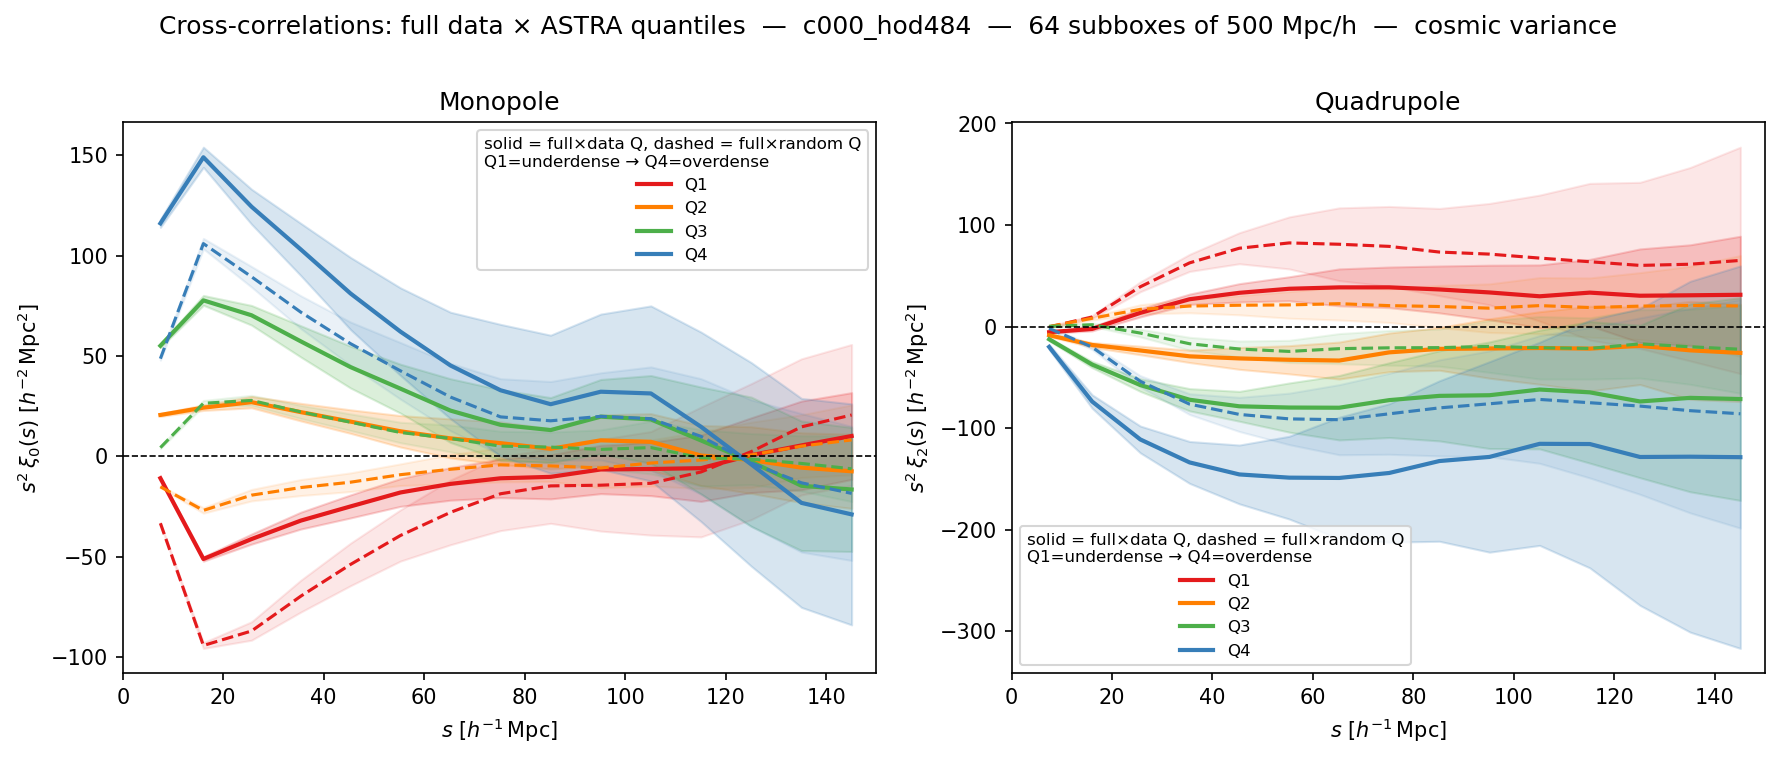
\includegraphics[width=0.95\textwidth]{subbox_cross_full_quantiles.png}
\caption{Cross-correlations of the full sample with each data quantile
(solid) and each random quantile (dashed).  Q2--Q4 cross zero at the
same scale as the full sample; Q1 approaches zero from below.}
\label{fig:cross}
\end{figure}

\section{Outlook}

Two points follow for our Fisher-matrix program.  First, the crossing
scale tracks the equality horizon, so it shifts with $\omega_{m}$; part
of the information in our $\omega_{c}$ derivatives will come from this
feature.  Second, because the crossing is invariant under
scale-independent bias, any future displacement of the quantile crossings
relative to the full sample would be a clean detection of scale-dependent
environmental bias, not a systematic error.

\begin{thebibliography}{9}

\bibitem{prada2011}
F.~Prada, A.~Klypin, G.~Yepes, S.~E.~Nuza, S.~Gottl\"ober,
\emph{Measuring equality horizon with the zero-crossing of the galaxy
correlation function}, arXiv:1111.2889 (2011).

\bibitem{anselmi2016}
S.~Anselmi, G.~D.~Starkman, R.~K.~Sheth,
\emph{The linear point: a cleaner cosmological standard ruler},
arXiv:1703.01275 (2017).

\bibitem{anselmi2018}
S.~Anselmi et al.,
\emph{Galaxy Correlation Functions Provide a More Robust Cosmological
Standard Ruler}, Phys.\ Rev.\ Lett.\ 121, 021302 (2018).

\bibitem{maksimova2021}
N.~A.~Maksimova et al.,
\emph{AbacusSummit: a massive set of high-accuracy, high-resolution
N-body simulations}, MNRAS 508, 4017 (2021).

\bibitem{landy1993}
S.~D.~Landy, A.~S.~Szalay,
\emph{Bias and variance of angular correlation functions},
ApJ 412, 64 (1993).

\bibitem{sinha2020}
M.~Sinha, L.~H.~Garrison,
\emph{Corrfunc: a suite of blazing fast correlation functions on the CPU},
MNRAS 491, 3022 (2020).

\end{thebibliography}

\end{document}
